\section{An illustrative example}
\label{Buildingblocks}
We illustrate the tradeoffs involved in implementing a packet-processing
pipeline on general-purpose
hardware, using an example of the L2 packet forwarding application.
At the high-level specification, the application involves input streams
of packets (one stream per input NIC) converging
to a processing node that looks up the packets' MAC addresses (source
and destination)
to index locally-stored lookup tables, to decide the destination of the packet, and
output streams of packets (one stream per output NIC) emerging out of
the processing node. We use
this simple application to illustrate the performance implications of
scheduling and prefetching decisions made by the compiler. We focus on performance
optimization for a single CPU core. Multi-queueing support in modern NICs
ensures that most applications can scale near-linearly with the number of cores.
\begin{figure}[ht]
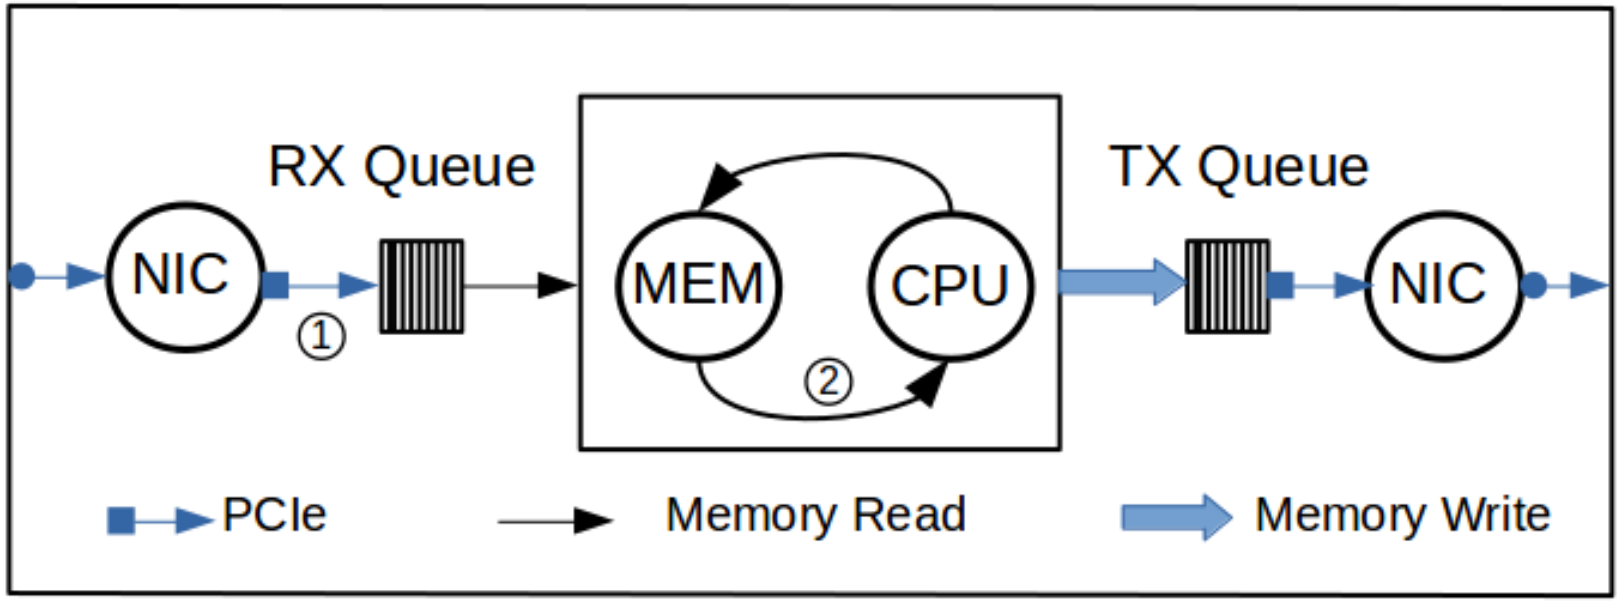
\includegraphics[width = \linewidth]{Figures/queuing.png}
\caption{Packet Processing Pipeline}
\label{fig:overviewfigure}
\end{figure}


We first discuss the characteristics of the underlying hardware.
Three components of a general-purpose architecture, are most critical to the performance of the
packet-processing
application: NIC subsystem, CPU, and Memory subsystem. Figure~\ref{fig:overviewfigure}
illustrates the data-flow at the hardware level. The NIC is involved in reading the packets
off the wire and storing them into main memory. In our experiments, a NIC's input bandwidth
is upper-bounded by 10Gbps, however, its bandwidth to memory is usually much higher\footnote{The
total PCIe bandwidth to main memory in our experiments
is around 8 GT/s, which gets shared across multiple NICs. For
all our experiments, except one (IPv4), the total PCIe bandwidth remains unsaturated.}. The latency
from NIC to main memory is usually long (i.e., the NIC-memory DMA interface is a high-bandwidth
high-latency interface), and so it is important to allow multiple
packets in flight from NIC to memory, to ensure effective bandwidth utilization across the
NIC-memory DMA interface. To realize this parallelism, we need {\em batching}, by ensuring
that multiple
packets are consumed/produced to the NIC's ring buffer in one shot. This allows the NIC to initiate
multiple PCIe transactions in parallel, thus hiding the round-trip NIC-memory latency. This
available parallelism at the NIC-memory interface is labeled as \textcircled{1}
in Figure~\ref{fig:overviewfigure}.

The next step in each packet processing pipeline is the actual logic.
Some applications are CPU-bound (involve
significant processing time), and others are memory-bound (involve significant cache-misses
and round trips to main memory). If an application is CPU bound, we cannot do much, and rely
on the underlying C compiler to tighten the code, and extract the SIMD and ILP parallelism. If
the application is memory-bound however, our code generator needs to exploit the
available memory-level parallelism.

The CPU-memory interface is also a high-bandwidth high-latency interface. CPUs allow multiple
memory requests to be in flight, by using MSHRs (miss-status handling registers) to store the
state of in-flight memory requests. Previous work on comparing CPU and GPU performance for
packet-processing pipelines \cite{189006} highlighted the importance of exploiting
memory-level parallelism in these workloads.
An out-of-order superscalar CPU executes a {\em window} of instructions in parallel.
Thus, a CPU can issue multiple main-memory requests in parallel, only if the consecutive memory
requests happen to be within a single instruction window. Kalia et. al. \cite{189006}
achieve this by {\em statically context-switching} among multiple threads, on each
expensive memory access. They relied on the programmer to manually annotate the expensive
memory accesses (the ones that are likely to result in a cache-miss) by hand.

We show that memory-level parallelism can be exploited through {\em sub-batching} (a sub-batch
is created within a larger batch that was required to efficiently NIC-memory bandwidth), for this
CPU-memory interface (\textcircled{2} in Figure~\ref{fig:overviewfigure}). Sub-batching
involves processing multiple packets (of sub-batch size) at
each step of the processing logic.
Sub-batching ensures that multiple independent lookups (if any) can be close-enough, such that
memory-level parallelism gets exploited.
Both batching and sub-batching, are
loop-fission transformations \cite{loop_fission}, when viewed as a compiler optimization.
Figures~\ref{fig:loop_fission_batch}~and~\ref{fig:loop_fission_subbatch} show
the batching and sub-batching transformations respectively. We use $B$
to denote the batch-size, and $b$ to denote the sub-batch-size.

\begin{figure}[ht]
\begin{small}
\begin{tabular}[b]{l|l}
sub\hspace{0.2cm}{\bf app} \{ &  sub\hspace{0.2cm}{\bf app} \{\\
\hspace{0.3cm}for (i = 0; i < B; i++) \{ &\hspace{0.3cm}for (i = 0; i < B; i++)\\
\hspace{0.6cm}p = read\_from\_input\_NIC(); &\hspace{0.6cm}p[i] = read\_from\_input\_NIC();\\
\hspace{0.6cm}p = process\_packet(p); & \hspace{0.3cm}for (i = 0; i < B; i++)\\
\hspace{0.6cm}write\_to\_output\_NIC(p); & \hspace{0.6cm}p[i] = process\_packet(p[i]);\\
\hspace{0.3cm}\} &\hspace{0.3cm}for (i = 0; i < B; i++)\\
&\hspace{0.6cm}write\_to\_output\_NIC(p[i]);\\
&\}\\
%&
%\mbox{
%hello
%\begin{verbatim}
%  for (i = 0; i < B; i++) {
%  }
%  for (i = 0; i < B; i++) {
%  }
%}
%\end{verbatim}
%}
\end{tabular}
\end{small}
\caption{\label{fig:loop_fission_batch} Batching.}
\end{figure}

\begin{figure}[ht]
\begin{small}
\begin{tabular}[b]{l|l}
sub\hspace{0.2cm}{\bf process\_packet}(p) \{ & sub\hspace{0.2cm}{\bf process\_packet}(p) \{\\
\hspace{0.3cm}for (i = 0; i < B; i++) \{ &\hspace{0.3cm}for (i = 0; i < B; i+=b) \{\\
\hspace{0.3cm}t1 = lookup\_table1(p[i]); &\hspace{0.6cm}for (j = i; j < i+b; j++)\\
\hspace{0.3cm}t2 = lookup\_table2(p[i], t1); & \hspace{0.9cm}t1[j-i] = lookup\_table1(p[j]);\\
\hspace{0.3cm}\ldots &\hspace{0.6cm}for (j = i; j < i+b; j++)\\
\} & \hspace{0.9cm}t1[j-i] = lookup\_table2(p[j], t1[j-i]);\\
&\hspace{0.6cm}\ldots\\
&\hspace{0.3cm}\}\\
&\}\\
\end{tabular}
\end{small}
\caption{\label{fig:loop_fission_subbatch} Sub-batching, within {\tt process\_packet}.}
\end{figure}


%In this work, we are exploring batching and prefetching, and in the next subsections, we will be writing about the relation of batching and prefetching with NIC, CPU, and Memory. These subsystems can work in parallel and batching \& prefetching can be used to improve the application performance.

%CPU can perform out of the order execution when memory subsystem is busy fetching the data. We can exploit this fact to make CPU and memory subsystem work in parallel. Prefetching works more effectively when it is associated with batching. With proper batch size, we are making sure that CPU has enough work to do while memory subsystem is bringing the data into the cache. Detailed description about batching and prefetching is in section \ref{iobatching}, \ref{computationbatching}, and \ref{prefetching}.

%\subsection{Packet Processing Pipeline}
%\label{overview}
%There are mainly three stages in the network packet processing flow: Receive, Process, Transmit.
% \begin{figure}[ht]
% 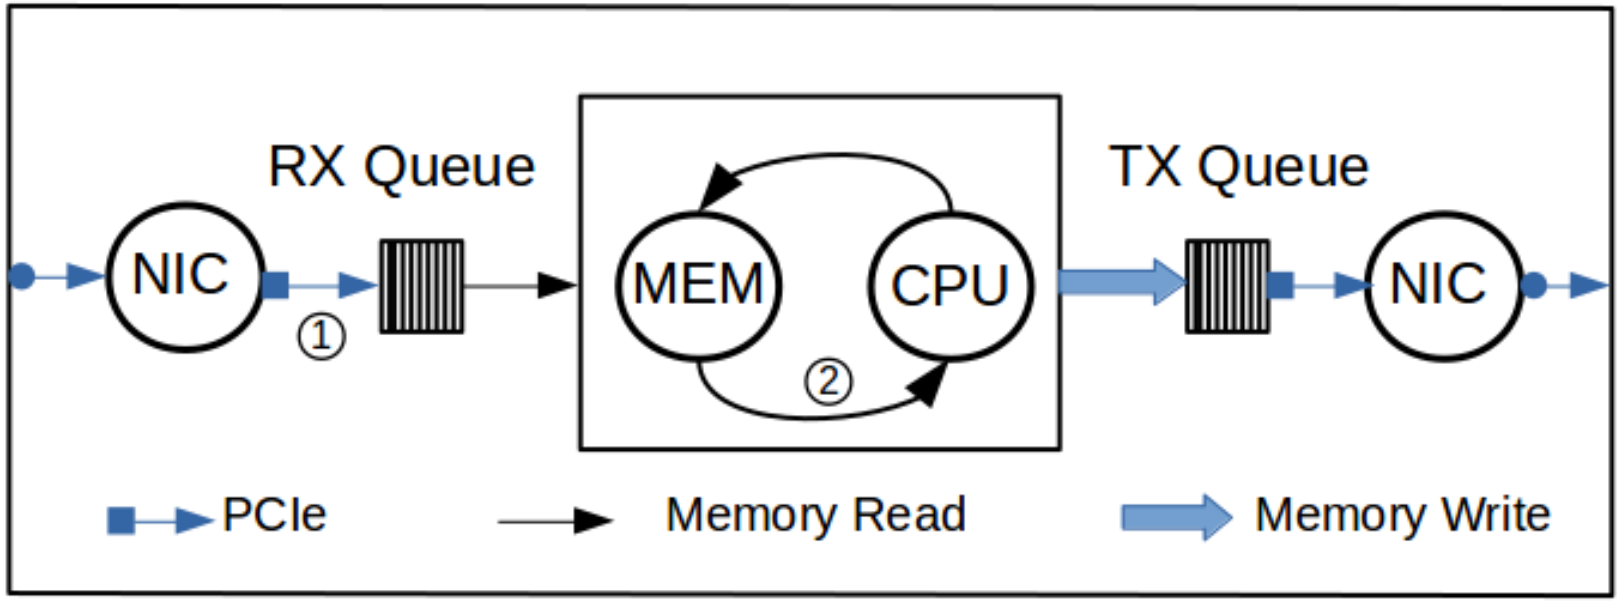
\includegraphics[width = \linewidth]{Figures/queuing.png}
% \caption{Packet Processing Pipeline}
% \label{fig:overviewfigure}
% \end{figure}
%\\
%\textbf{Receive:} After receiving data from the physical layer, NIC puts the data in the buffer and then DMA engine transfers it in main memory through PCIe. Driver maintains the queue for received packets and passes the ownership to the application by reflecting it in the descriptors. When the application makes a function call to receive packets, poll mode driver(PMD) passes the packets to the userspace application. DPDK has library functions to RX and TX packets in batches. Descriptors are shared by NIC and PMD as a Single  Producer Single Consumer Queue and they both polls other ends of it independently.
%\\
%\textbf{Process:} Lookup based applications are very common in packet processing and we are more interested in such applications. The typical flow for such application involves header extraction, lookup based on header field(s), and transmission based on the lookup result.
%\\
%\textbf{Transmit:} This stage is very similar to receive stage in reverse direction.
%
%\subsection{I/O Batching}
%\label{iobatching}
%It can be noted in the section \ref{overview} that RX and TX of a packet is a costly process. Transferring the descriptors and packet from NIC to memory incurs overheads for each PCI transaction. For RX and TX of each packet, there is a DMA overhead, PCIe overhead, and packet buffer \& descriptors management overhead. These overheads can be amortized among packets by transferring them in batches. We are using DPDK based poll mode driver which supports IO batching and has implemented the batched receive and transmit of packets in an efficient way by using vector instructions.
%
%\subsection{Computation Batching}
%\label{computationbatching}
%For each packet processing, there is a cost involved, an application does some sort of bookkeeping, executes many functions based on the application flow, and accesses various data structure. All this cost can be amortized among packets if we are doing all these operations in batches. In case of computation batching, all the packets pass through one stage before moving to the next stage. Instead of calling a function batch time, each function is called once and all the packets in the batch are processed together. It reduces the function call overhead. Data and instruction locality also increases because CPU executes the same portion of the code and accesses the same data structure for batch number of times before moving to next stage. Batching also allows the use of vector instructions to make packet processing more efficient.

%\subsection{Prefetching}
%\label{prefetching}
%Software prefetching is an old concept and has been used extensively to improve the performance for memory-bound applications. In Figure \ref{overviewfigure}, we are showing memory subsystem as one component, however, CPU can issue multiple memory accesses and memory subsystem can fetch \#MSHRs requests in parallel. Prefetch allows the application to use memory and CPU in parallel e.g. CPU can do its work while the memory system is bringing data into L1 cache. If we know that some data will be used later in the program, it can be prefetched by the prefetch instruction. In Algorithm \ref{lookup-algo} we are showing how prefetch can be used for lookup based network application. In line \ref{hash-lookup-line} we need bucket where the key is present. If we remove prefetch instruction in Line \ref{prefetch-line} CPU will stall at Line \ref{hash-lookup-line} if the bucket is not present in L1 cache. To avoid the stall we can prefetch the bucket in the first loop. This will reduce the total stall time and the performance of the application will increase.

Sub-batching hides the CPU-memory latency. We further improve it by using the 
x86 {\em prefetch} instruction for future packets.
The prefetch instruction allows the hardware to differentiate a memory
request that is likely to be used in future, from a memory request that is likely
to be used immediately (fetch), and allows better scheduling of resources by hardware.
Algorithm~\ref{algo:prefetch}
shows the example prefetching code used for the hash-lookup in the L2 forwarding example.

\begin{algorithm}[H]
 \caption{HASH LOOKUP}
 \label{algo:prefetch}
 \begin{algorithmic}[1]
 \For{$i \leftarrow 1$ To $Batch Size$}
     \State key-hash[i] = extract key and compute hash;\Comment{$C_K$} \label{hash-compute-line}
     \State prefetch(bucket-for-key-hash(key-hash[i]));\Comment{$C_P$} \label{prefetch-line}
 \EndFor
 \\
 \For{$j \leftarrow 1$ To $Batch Size$}
     \State value[j] = hash-lookup(key-hash[j]);\Comment{$C_L$} \label{hash-lookup-line}
 \EndFor
 \end{algorithmic}
\end{algorithm}
Notice that sub-batching is dependent upon batching, in that, the sub-batch-size can only be smaller than the batch-size. Thus, if there is no
batching, there can be no sub-batching. We find that the optimal sub-batch-size is often less than the
optimal batch-size.

Finally, the processed packets are transmitted to the output NICs. Assuming uniform distribution of output packets
across output NICs, we expect
the utilization at the output memory-NIC DMA interface to be similar to the utilization of the input NIC-memory DMA
interface.

We evaluate the effectiveness of the batching and sub-batching transformations, and systematically explore
the solution space to search for the optimal values of $B$ (batch-size) and $b$ (sub-batch-size), in our experiments.

%\textbf{Prefetch Distance and Batch Size:}
%\label{subbatching}
%Given that $C_K$, $C_P$, and $C_L$ are the number of cycles needed to calculate the hash, issue the prefetch, and lookup the value respectively. We are issuing prefetch $(C_K + C_P) * (BatchSize-i) + C_L*(i-1)$ number of cycles before, where $i$ is packet number. However, all the prefetches can't work in parallel and maximum \#MSHR(Miss Status Handling Registers) prefetch instructions work in parallel. So effective prefetch distance is defined by the number of free MSHRs.
%
%Efficient use of Software prefetching is highly dependent on right prefetch distance. Prefetch distance can be explained as CPU cycles between the prefetch instruction and the instruction where data is being used. If the prefetch distance is very small then we won't be able to reduce the memory stall and there is an additional overhead of issuing prefetch instruction. If the prefetch distance is too high then the data might not be in the cache when the application needs it. For example, if the values of $C_K$ and $C_L$ are large and we are using large batch size then prefetch distance would be more and we might not be able to find the data when needed. In such cases, we can reduce the batch size to make the prefetch distance more precise. We can form the sub-batches at lookup stage instead of changing the batch size at the application level.
%
%\section{Relation between Batching and Prefetching}
%\label{optimalbatchsize}
%Batching has been used extensively for network applications. In our knowledge, there is no model which can be used to find a relation between batching and prefetching. In this work, we have tried to formulate the correlation by including important parameters, which is generic enough to be used on any platform. We need to set the optimal batch size at three levels to make the application run efficiently, IO level, CPU level, and Memory level.
%
%\subsection{Mathematical Model}
%In this section, we are formulating the dependence between throughput and batch size. We are explaining the model form top to down to decide optimal batch size. Let
%\begin{align}
%B_{opt} &=  \text{arg}\,\max\limits_{(B_1, B_2)}\, (\Upsilon(B_1) , \Theta(B_2)) \label{bopt}
%\\
%\text{T} &= \frac{1}{\max (\Upsilon(B_1) , \Theta(B_2))} \label{overall_throughput}
%\end{align}
%\\
%where $\Upsilon(.)$ and $\Theta(.)$ represents I/O processing and compute processing, time at given batch size for one packet, respectively. $\text{T}$ is overall processing throughput in packets per second.\\ \\
%$\Upsilon(.)$ will depend on PCI bandwidth, PCI latency, NIC, DMA engine etc.
%\begin{equation} 
%\label{nic_throughput}
%\Upsilon(B) = \Psi(\textrm{PCI, NIC, DMA engine, others})
%\end{equation}
%$\Theta(.)$ is directly proportional to total cycles CPUs takes to process a single packet. This includes cycles wasted by CPUs to wait for data to come from memory system. 
%\\
%\begin{equation} 
%\label{compute_througput}
%\Theta(B) \propto \Delta_{compute}(B) + \frac{\Delta_{stall}(B)}{B}
%\end{equation}
%Given batch size $B$, $\Delta_{compute}(B)$ represents number of cycles CPU is busy doing computation for a single packet and $\Delta_{stall}(B)$ represents number of cycles CPU  is waiting for memory operations to complete for all $B$ packets. As explained in Section \ref{prefetching}  and \ref{subbatching} CPU may stall if it needs a data which is not present in L1 cache. $\Delta_{compute}(.)$ can also vary with batch size due to increase in data and instruction locality in the memory system.
%\\
%$\Delta_{compute}(.)$ can be broken down into two useful terms, representing cycles which gets amortized and cycles which doesn't gets amortized due to batching.
%\\
%\begin{equation} 
%\label{cycles_compute}
%\Delta_{compute}(B) = \frac{\Delta_{shared}(B)}{B} + \Delta_{necessary}(B)
%\end{equation}
%Given batch size $B$, $\Delta_{necessary}(B)$ is unamortizable work that needs to be done per packet and $\Delta_{shared}(B)$ is work that is done once per batch and not per packet. For example, overheads for function calls gets amortized among the batch whereas packet header extraction needs to be done for every packet, thus, not amortizable.
%\\
%Average cycle stall per packet is the difference of average cycles memory system takes to bring data into caches for one packet and useful computation done on an average during that time for a packet.
%\\
%\begin{equation}
%\label{cycles_stall}
%\frac{\Delta_{stall}(B)}{B} = \Delta_{fetch}(B) - \frac{\Delta_{hide}(B)}{B}
%\end{equation}
%where $\Delta_{stall}(B)$ is the average latency of fetching data from memory system into caches and $\Delta_{hide}(B)$ is the work done while memory system is bringing data into caches. In Algorithm \ref{lookup-algo} CPU is doing work for another packet in batch while memory subsystem is prefetching the required data. As explained in Section \ref{prefetching}, prefetching will reduce the overall stall time.
%
%\textbf{Summary:} To get the maximum throughput, we need to set the optimal batch size at all the levels. Our aim is to find out the optimal batch size at IO level, CPU level, and Memory level. We are assuming that packets are coming with a uniform rate. IO batch size is dependent on PCIe bandwidth and availability of on-die memory space, as far as we are using these resources efficiently we can keep the batch size minimum. At CPU, optimal batch size is dependent on the rate at which it is processing the packets and if the NIC is able to accumulate the Batch Size number of packets in that time then the batch size is optimal, until then we can increase the batch size. Another important factor which we need to consider is the optimal use of cache, if we are using large batch size then packet data, descriptors, and table entries will compete for the cache and this will result in throughput degradation. At Memory, our goal is to minimize the stall cycles and the batch size which is giving the right prefetch distance for the prefetches would be the optimal memory level batch size. In Experiment \ref{batchvstable} we are explaining the results with the help of this model.
